%% (pdf)latex + bibtex + (pdf)latex + (pdf)latex [+ preview]
%%  F6 + F11 + F6 + F6 [+ F7]

%% abtex2-modelo-trabalho-academico.tex, v-1.9.6 laurocesar
%% Copyright 2012-2016 by abnTeX2 group at http://www.abntex.net.br/ 
%%
%% This work may be distributed and/or modified under the
%% conditions of the LaTeX Project Public License, either version 1.3
%% of this license or (at your option) any later version.
%% The latest version of this license is in
%%   http://www.latex-project.org/lppl.txt
%% and version 1.3 or later is part of all distributions of LaTeX
%% version 2005/12/01 or later.
%%
%% This work has the LPPL maintenance status `maintained'.
%% 
%% The Current Maintainer of this work is the abnTeX2 team, led
%% by Lauro César Araujo. Further information are available on 
%% http://www.abntex.net.br/
%%
%% This work consists of the files abntex2-modelo-trabalho-academico.tex,
%% abntex2-modelo-include-comandos and abntex2-modelo-references.bib
%%

% ------------------------------------------------------------------------
% ------------------------------------------------------------------------
% abnTeX2: Modelo de Trabalho Academico (tese de doutorado, dissertacao de
% mestrado e trabalhos monograficos em geral) em conformidade com 
% ABNT NBR 14724:2011: Informacao e documentacao - Trabalhos academicos -
% Apresentacao
% ------------------------------------------------------------------------
% ------------------------------------------------------------------------

\documentclass[
	% -- opções da classe memoir --
	12pt,				% tamanho da fonte
	openright,			% capítulos começam em pág ímpar (insere página vazia caso preciso)
    oneside,			% para impressão em recto e verso. Oposto a oneside
	a4paper,			% tamanho do papel. 
	% -- opções da classe abntex2 --
	%chapter=TITLE,		% títulos de capítulos convertidos em letras maiúsculas
	%section=TITLE,		% títulos de seções convertidos em letras maiúsculas
	%subsection=TITLE,	% títulos de subseções convertidos em letras maiúsculas
	%subsubsection=TITLE,% títulos de subsubseções convertidos em letras maiúsculas
	% -- opções do pacote babel --
	english,			% idioma adicional para hifenização
	french,				% idioma adicional para hifenização
	spanish,			% idioma adicional para hifenização
	brazil				% o último idioma é o principal do documento
	]{abntex2}


% ---
% Pacotes básicos 
% ---
\usepackage{lmodern}			% Usa a fonte Latin Modern			
\usepackage[T1]{fontenc}		% Selecao de codigos de fonte.
\usepackage[utf8]{inputenc}		% Codificacao do documento (conversão automática dos acentos)
\usepackage{lastpage}			% Usado pela Ficha catalográfica
\usepackage{indentfirst}		% Indenta o primeiro parágrafo de cada seção.
\usepackage{color}				% Controle das cores
\usepackage{graphicx}			% Inclusão de gráficos
\usepackage{microtype} 			% para melhorias de justificação
% ---

\graphicspath{{../figuras}}

% ---
% Pacotes adicionais, usados apenas no âmbito do Modelo Canônico do abnteX2
% ---
\usepackage{lipsum}				% para geração de dummy text
% ---

% ---
% Pacotes para escrita matemática
% ---
\usepackage{amsmath}

\usepackage{amssymb}	 % qed
\usepackage{amsthm}      % Teoremas

%\declaretheorem[style=definition,name=Definição,parent=chapter,qed=\textemdash]{definicao}
%\declaretheorem[style=plain, name=Teorema]{teorema}
%\declaretheorem[style=plain, name=Axioma,qed=\textnormal{\textemdash}]{axioma}
%\declaretheorem[style=plain, name=Lema]{lema}
\newtheorem{teorema}{Teorema}
\newtheorem{lema}{Lema}
\newtheorem{definicao}{Definição}

% Resetar o numberador de lemas no fim de todo capítulo
% Isso faz com que a numeração seja indexada por capítulos e não
% pelo documento todo
\numberwithin{lema}{chapter}
% Idem ao de cima, com teoremas/axiomas/definições
\numberwithin{teorema}{chapter}
\numberwithin{definicao}{chapter}
%\numberwithin{axioma}{chapter}
%\numberwithin{definicao}{chapter}
% Idem aos anteriores com o ambiente figure
\numberwithin{figure}{chapter}

% PGF
\usepackage{pgf,tikz,pgfplots}
\pgfplotsset{compat=1.15}
\usepackage{mathrsfs}
\usetikzlibrary{arrows}
\usepackage{standalone}

% ---
% Pacotes de citações
% ---
\usepackage[brazilian,hyperpageref]{backref}	 % Paginas com as citações na bibl
\usepackage[alf]{abntex2cite}	% Citações padrão ABNT
% --- 
% CONFIGURAÇÕES DE PACOTES
% --- 

% ---
% Configurações do pacote backref
% Usado sem a opção hyperpageref de backref
\renewcommand{\backrefpagesname}{Citado na(s) página(s):~}
% Texto padrão antes do número das páginas
\renewcommand{\backref}{}
% Define os textos da citação
\renewcommand*{\backrefalt}[4]{
	\ifcase #1 %
		Nenhuma citação no texto.%
	\or
		Citado na página #2.%
	\else
		Citado #1 vezes nas páginas #2.%
	\fi}%
% ---

% ---
% Informações de dados para CAPA e FOLHA DE ROSTO
% ---
\titulo{Cálculo Variacional}
\autor{EDUARDO JOSÉ DE OLIVEIRA}
\local{ANÁPOLIS}
\data{2019}
\orientador{Prof. Me. Tiago de Lima Bento Pereira}
%\coorientador{Titulação e Nome do coorientador}
\instituicao{%
Universidade Estadual de Goiás
  \par
Câmpus Anápolis de Ciências Exatas e Tecnológicas Henrique Santillo
  \par
Curso de Matemática}
\tipotrabalho{Trabalho de Curso (Graduação)}
% O preambulo deve conter o tipo do trabalho, o objetivo, 
% o nome da instituição e a área de concentração 
\preambulo{Trabalho de Curso (TC) apresentado a Coordenação Adjunta de TC, como parte dos requisitos para obtenção do título de Graduado no Curso de Matemática da Universidade Estadual de Goiás.} %sob a orientação do Professor(a) titulação e nome do professor(a).}
% ---


% ---
% Configurações de aparência do PDF final

% alterando o aspecto da cor azul
\definecolor{blue}{RGB}{41,5,195}

% informações do PDF
\makeatletter
\hypersetup{
     	%pagebackref=true,
		pdftitle={\@title}, 
		pdfauthor={\@author},
    	pdfsubject={\imprimirpreambulo},
	    pdfcreator={LaTeX with abnTeX2},
		pdfkeywords={abnt}{latex}{abntex}{abntex2}{trabalho acadêmico}, 
		colorlinks=false,       		% false: boxed links; true: colored links
    	linkcolor=blue,          	% color of internal links
    	citecolor=blue,        		% color of links to bibliography
    	filecolor=magenta,      		% color of file links
		urlcolor=blue,
		bookmarksdepth=4
}
\makeatother
% --- 

% --- 
% Espaçamentos entre linhas e parágrafos 
% --- 

% O tamanho do parágrafo é dado por:
\setlength{\parindent}{1.3cm}

% Controle do espaçamento entre um parágrafo e outro:
\setlength{\parskip}{0.2cm}  % tente também \onelineskip

% ---
% compila o indice
% ---
\makeindex
% ---
\usepackage{matematicaCCETrelatorio} %MEU 
\usepackage{helvet} %Meu importa uma fonte nova "sem serifa"
\usepackage{pdfpages}

\renewcommand{\ABNTEXsectionfontsize}{\normalsize}
\usepackage{enumitem}
\usepackage{geometry}
\newgeometry{a4paper, head=95pt, left=3cm, top=4cm, right=2cm, bottom=2cm, foot=100pt}
\usepackage{multirow} % Usado para compilar a tabela da sessão "Atividades Cumpridas do Cronograma do TC"

\newcommand{\CompromissoItemOptions}{
	\begin{center}
		\begin{tabular}{c c c}
			(\hspace{0.3cm}) Sim \hspace{1.5cm}  & (\hspace{0.3cm}) Parcialmente \hspace{1.5cm} & (\hspace{0.3cm}) Não
		\end{tabular}
	\end{center}
}

\newcommand{\notitleitem}[1]{
	\item[\refstepcounter{enumi}\textbf{#1}]
}

\newcounter{apendice}[section]

\newcommand{\referencias}{\notitleitem{Referências}}
\newcommand{\apendice}[1]{
	\refstepcounter{apendice}
	\notitleitem{Apêndice~\Alph{apendice}:} #1
}

\renewcommand{\bibsection}{%
    %\chapter*{\bibname}
    \section*{REFERÊNCIAS}
    \bibmark
    %\ifnobibintoc\else
    %\phantomsection
    %\addcontentsline{toc}{chapter}{\texorpdfstring{\MakeTextUppercase{\bibname}}{\bibname}}
    %\fi
    \prebibhook
}

\makeoddhead{abntchapfirst}{}{}{}
\makeoddhead{abntheadings}{\ABNTEXfontereduzida\textit\rightmark}{}{}

% ----
% Início do documento
% ----
\begin{document}

% Seleciona o idioma do documento (conforme pacotes do babel)
%\selectlanguage{english}
\selectlanguage{brazil}

% Retira espaço extra obsoleto entre as frases.
\frenchspacing 

\pretextual
{
	% ---
	% Capa
	% ---
	\imprimircapa
	\clearpage
}
%
% Relatório
%
\pagestyle{ueg_mat_heading}
{
	
	%
	% Estrutura do Trabalho de Curso
	%
	\section*{ESTRUTURA DO TC}

	%Definir a estrutura inicial do TC, ou seja, quantos e quais capítulos estão previstos e o que poderá ter neste trabalho. Essa estrutura pode ser ajustada no decorrer do desenvolvimento do trabalho de curso.
	A estrutura prevista para este trabalho de curso é a seguinte:
	
	%
	% -> Ambiente Enumerate contendo a estrutura dos capítulos do TC
	%
	\begin{enumerate}[align=left,leftmargin=*,label=\textbf{Capítulo \arabic*}:]
		\item Introdução
		\item Contexto Histórico
		\item Cálculo Variacional
		\item Aplicações
		% ...
		\referencias
		\apendice {Regra de Leibniz}
	\end{enumerate}

	%
	% Atividades cumpridas do cronograma
	%
	\section*{ATIVIDADES CUMPRIDAS DO CRONOGRAMA DO TC}

	%Neste item devem ser assinaladas com um \textbf{X} as atividades que já foram desenvolvidas para a realização do TC. Lembre-se que essas atividades foram listadas no Projeto de Trabalho de Curso, no entanto, podem ser feitas alterações nessas atividades, incluindo ou excluindo algumas dessas atividades.
	
	% Use o seguinte pacote requerido no preâmbulo do seu documento:
% \usepackage{multirow} % (Inserido no preâmbulo do modelo do CCET matemática)
% \usepackage{graphicx}

\begin{table}[h!]
\centering
\resizebox{\textwidth}{!}{%
\begin{tabular}{|l|l|l|l|}
\hline
\multirow{2}{*}{Atividades desenvolvidas}        & \multicolumn{3}{c|}{\begin{tabular}[c]{@{}c@{}}Bimestre\\ de\\ \imprimirdata\end{tabular}} \\ \cline{2-4} 
                                                 & \multicolumn{1}{c|}{1\textsuperscript{o}}        & \multicolumn{1}{c|}{2\textsuperscript{o}}        & 3\textsuperscript{o}                             \\ \hline
Levantamento Bibliográfico                       & \multicolumn{1}{c|}{X}        & \multicolumn{1}{c|}{X}        & \multicolumn{1}{c|}{X}        \\ \hline
Redação do Relatório do Trabalho de Curso I.     &                               & \multicolumn{1}{c|}{X}        & \multicolumn{1}{c|}{X}        \\ \hline
Apresentação do relatório do Trabalho de Curso I &                               &                               & \multicolumn{1}{c|}{X}        \\ \hline
Aplicação no ensino médio                        &                               &                               &                               \\ \hline
Estudo dos recursos computacionais               &                               &                               &                               \\ \hline
Aplicação Física                                 &                               &                               &                               \\ \hline
Redação do Relatório do Trabalho de Curso II     &                               &                               &                               \\ \hline
Revisão                                          &                               &                               &                               \\ \hline
Revisão Final                                    &                               &                               &                               \\ \hline
\end{tabular}%
}
\end{table}

% Observação:
% Essa tabela foi gerada utilizando a ferramenta online:
% 	   https://www.tablesgenerator.com
%
% O arquivo original dela está na pasta "raw/tabela_exemplo_tc.tgn".
% Importe no site "tablesgenerator" usando "File -> Load Table". % insere o conteúdo do arquivo "tabela_cronograma.tex" apenas para simplificar a exibição\edição destes documentos
	
	%
	% Resultados Parciais
	%
	\section*{RESULTADOS PARCIAIS}
	
	Os resultados parciais são apresentados nas páginas subsequentes.
}
\clearpage
%
% Texto dos resultados parciais
%
% retoma os estilos de cabeçalho para o abntex
\thispagestyle{abntheadings}
\textual
{
	\chapter{Contexto Histórico}

Para elucidar a história do Cálculo Variacional é importante mostrar um pouco da história dos máximos e mínimos de funções, problema pertinente ao cálculo diferencial, para, então, adentrar aos problemas de máximos e mínimos de funcionais, problema pertinente ao cálculo variacional.

\section{Máximos e Mínimos}

Os problemas de máximo e mínimo são corriqueiros na vida cotidiana, por exemplo, quando se quer encontrar o caminho com menor distância entre dois lugares para se caminhar uma menor distância, dentre vários outros problemas mais elaborados. Para esse exemplo específico não é necessário o uso de matemática avançada, porém, quanto mais complexidades são adicionadas aos problemas, mais a matemática é necessária para a resolução, exata ou aproximada. Para simplificar estes processos, surgem os métodos para o cálculo de máximos e mínimos das funções.

Uma das primeiras formulações matemáticas próxima das atuais para os problemas de máximos e mínimos foi feita por Pierre de Fermat (1601-1665) em 1629 considerando curvas $y=f(x)$. Ele fez comparações de $f(x)$ e $f(x+E)$ para pontos próximos. Esses valores geralmente são diferentes, porém, próximo de máximos ou mínimos a diferença se torna pequena. Deste modo, para achar os pontos de máximo ou mínimo, Fermat fazia $$\frac{f(x+E)-f(x)}{E}$$ e, após realizar a divisão, considerava $E=0$. Após considerar o valor de $E$ igual a $0$, Fermat igualava a expressão obtida a $0$, de onde conseguia extrair os valores das abscissas dos pontos de máximos e mínimos da função. \cite{boyer}

O que Fermat fez, de fato, foi igualar a primeira derivada de uma função a $0$. É importante ressaltar que esse método utilizado por Fermat veio antes mesmo da invenção do cálculo diferencial por Isaac Newton (1642-1727) em 1665-1666 e Gottfried Wilhelm Leibniz (1646-1716) em 1676, de forma independente. \cite{boyer}

\section{O Cálculo Variacional}

O ponto de partida do cálculo variacional se deu com Johann Bernoulli, em 1696, com a publicação do problema da braquistócrona no jornal científico \textit{Acta Eruditorium}. \cite{hist_courant}

O problema pode ser enunciado como:
\begin{citacao}
Sejam $A$ e $B$ dois pontos dados em um plano vertical. O problema da braquistócrona consiste em encontrar a curva que uma partícula M precisa descrever para sair de A e chegar em B no menor tempo possível, somente sob a ação da força da gravidade \cite[p. 3]{calcvar}.
\end{citacao}

O próprio Johann Bernoulli foi um dos matemáticos que solucionou o problema da braquistócrona. Ele retardou a publicação da sua solução para estimular os matemáticos do seu tempo a testarem suas habilidades nesse novo tipo de problema matemático \cite{hist_courant}. Além de Johann Bernoulli, soluções independentes foram encontradas por diversos matemáticos, como Jacob Bernoulli (1697), L'Hôpital (1697), Leibniz (1697), e Newton (1697) \cite{hist_still}.

A solução de Jacob Bernoulli considerava o aspecto da curva variável, sendo considerado o primeiro grande passo para o desenvolvimento do cálculo variacional \cite{hist_still}. Nesse problema, a quantidade a ser minimizada depende de uma curva e não apenas de uma váriavel real \cite{hist_courant}, diferentemente dos problemas relacionados ao cálculo diferencial, o que torna necessária a construção de novas ferramentas matemáticas. 

Os métodos para a resolução de problemas deste tipo eram específicos com adaptações para cada caso, sendo que os métodos gerais para a resolução só foram desenvolvidos com o envolvimento dos matemáticos Euler e Lagrange nos estudos desses problemas \cite{hist_courant}.


\chapter{Cálculo Variacional}

O problema pertinente ao cálculo variacional é o de encontrar uma função diferenciável até segunda ordem $y=y(x)$ satisfazendo $y(x_1)=y_1$ e $y(x_2)=y_2$, com $x_1$, $x_2$, $y_1$ e $y_2$ dados, minimizando ou maximizando a integral
\begin{equation}
	\int_{x_1}^{x_2} f(x,y,y')dx\text{.}
	\label{eqn:int_funcional}
\end{equation}

Para para encontrar a equação $y=y(x)$ procurada, são necessárias algumas ferramentas, dentre as quais a abordada neste estudo é a equação de Euler-Lagrange. Os conceitos, definições e resultados apresentados neste capítulo foram elaboradas segundo \citeonline{calcvar} e \citeonline{mefassan}.

\section{Equação de Euler-Lagrange}

De ínicio, é preciso demonstrar um lema que servirá como base para a dedução da equação de Euler-Lagrange.

\begin{lema}
\label{lema:cap_calcvar_lema_1}
Sejam $x_1 < x_2$ fixos e $G(x)$ uma função contínua particular para $x_1 \leqslant x \leqslant x_2$. Se $$\int_{x_1}^{x_2} \eta (x) G(x) dx = 0$$
para cada função diferenciável $\eta (x)$ tal que $\eta (x_1)=\eta (x_2)=0$, concluímos que $G(x)=0$, para todo $x$ de modo que $x_1 \leqslant x \leqslant x_2$.

\begin{proof}
Suponha que existe $\overline{x}$ tal que $x_1\ < \overline{x} < x_2$ e $G(\overline{x})\neq 0$. Podemos supor, sem perda de generalidade, que $G(\overline{x})>0$. Como $G$ é contínua, existe uma vizinhança $\overline{x_1} \leqslant \overline{x} \leqslant \overline{x_2}$ onde $G(x)>0$ em toda a vizinhança.

Podemos construir a seguinte função $\eta (x)$:
$$
\eta (x) = 
	\begin{cases}
		0 											& \mbox{para } x_1 \leqslant x < \overline{x_1}\\
		(x-\overline{x_1})^2(x-\overline{x_2})^2	& \mbox{para } \overline{x_1} \leqslant x \leqslant \overline{x_2}\\
		0											& \mbox{para } \overline{x_2} < x \leqslant x_2
	\end{cases}
$$
e então reescrever a integral do seguinte modo:
$$\int_{x_1}^{x_2}\eta (x) G(x)dx =\int_{\overline{x_1}}^{\overline{x_2}}(x-\overline{x_1})^2(x-\overline{x_2})^2G(x)dx\text{.}$$

Como $G(x) > 0$ em $\overline{x_1} \leqslant x \leqslant \overline{x_2}$, a integral do lado direito é estritamente positiva, contradizendo a hipótese. Portanto, não vale para todo $\eta (x)$, de onde $G(\overline{x})=0$. A demonstração considerando $G(\overline{x})<0$ é análogo.
\end{proof}
\end{lema}

Suponha $x_1$, $x_2$, $y_1$, $y_2$ dados, $f$ uma função de $x$, $y$ e $y'$ duas vezes diferenciável. É preciso construir uma família de funções aproximadoras, que será denotada por $Y(x)$. Essa família é definida por:
\begin{equation}\label{eqn:cap_calcvar_eq_approx}
	Y(x)=y(x)+\varepsilon \eta (x)\text{,}
\end{equation}
onde $\eta (x)$ é uma função diferenciável arbitrária para a qual $\eta (x_1)=\eta (x_2) = 0$. O número $\varepsilon$ é o parâmetro da família. É possível escrever, também, a derivada de $Y$ como
\begin{equation}\label{eqn:cap_calcvar_eq_approx_diff}
	Y'(x)=y(x)+\varepsilon \eta (x)\text{.}
\end{equation}

%\textit{\color{red} Inserir uma imagem da representação gráfica das famílias de funções aproximadoras.}

\begin{figure}[!h]
	\caption{Representação gráfica das funções aproximadoras.}
	\centering
	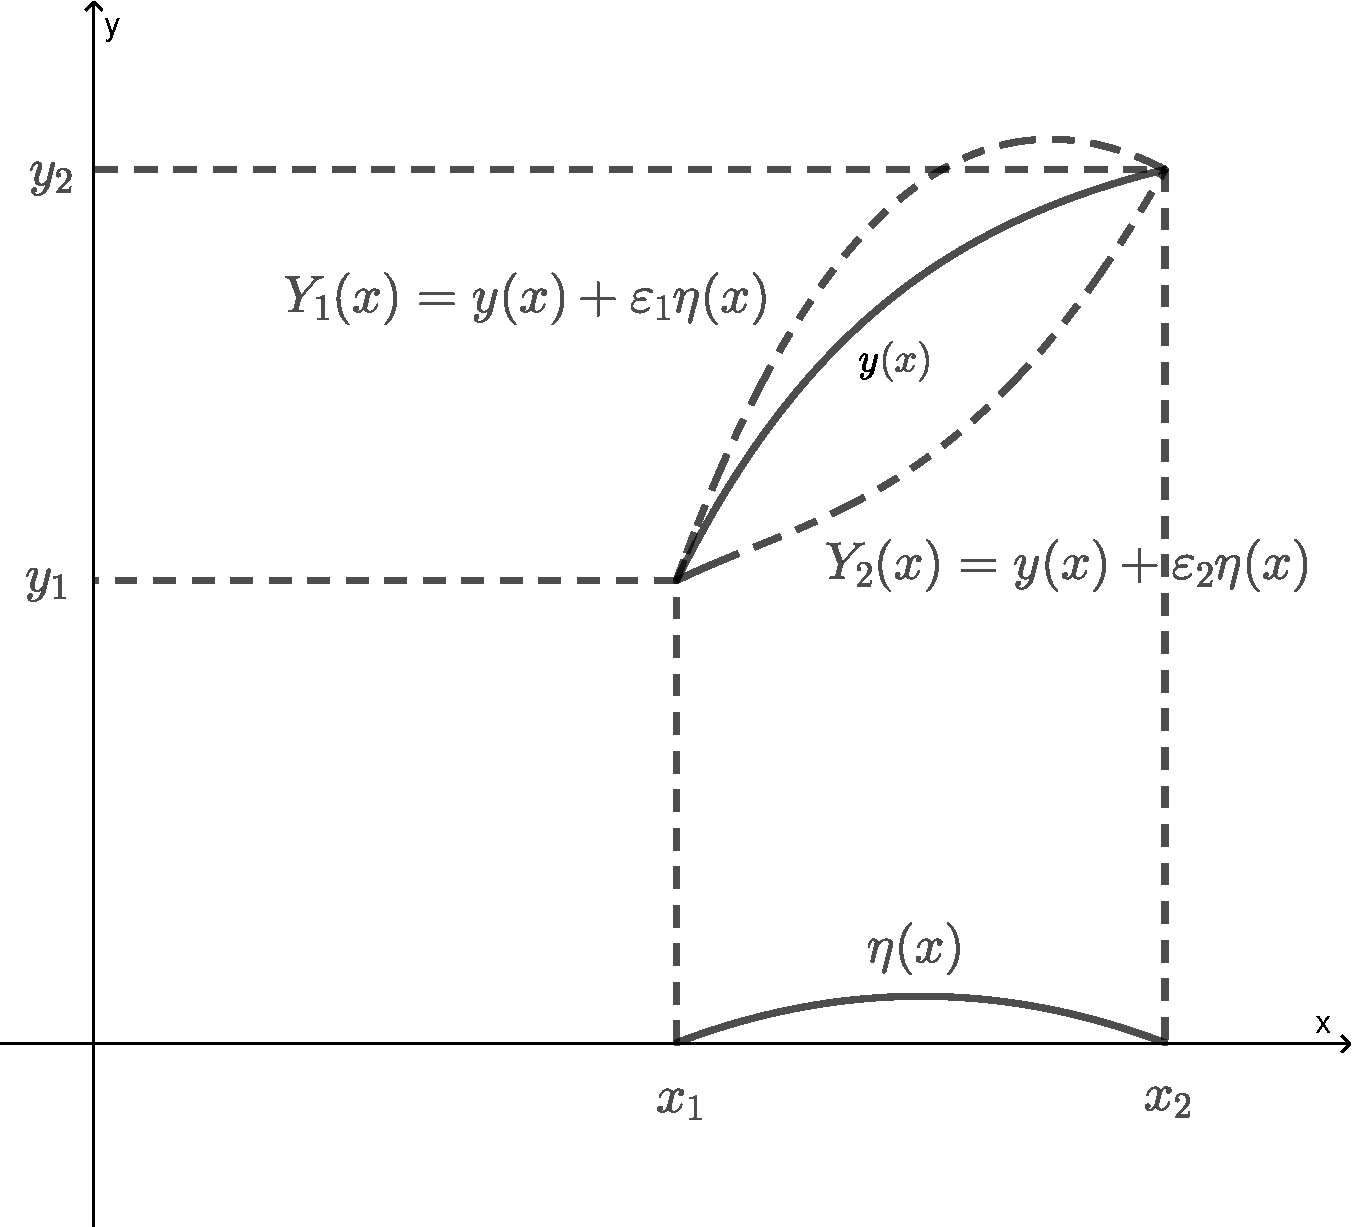
\includegraphics[width=0.5\textwidth, angle=0]{../figuras/cap_calcvar/figura_001.pdf}
	\label{fig:test_01}
	\legend{\ABNTEXfontereduzida Fonte: Elaborada pelo autor, 2019.}
\end{figure}

Reescrevendo a integral (\ref{eqn:int_funcional}) utilizando as funções aproximadoras definidas, tem-se
\begin{equation}\label{eqn:int_funcional_approx}
I(\varepsilon)=\int_{x_1}^{x_2}f(x, Y, Y')dx\text{.}
\end{equation}

Note que a função procurada $y(x)$ é o membro da família $Y(x)$ quando $\varepsilon = 0$. Ou seja, se $\varepsilon = 0$ pode-se substituir $Y$ e $Y'$ por $y$ e $y'$, respectivamente. Deste modo, a integral (\ref{eqn:int_funcional_approx}) fornece os mesmos extremos que a (\ref{eqn:int_funcional}) quando $\varepsilon=0$.

A condição necessária para que uma função de uma variável real tenha um extremo em algum ponto é que sua primeira derivada se anule nesse ponto. Então, é necessário que
\begin{equation}\label{eqn:cap_calcvar_condition}
I'(0)=0\text{.}
\end{equation}

Utilizando a Regra de Leibniz (Teorema \ref{teorema:regra_de_leibniz} do Apêndice \ref{apend:regra_de_leibniz}), a derivada de (\ref{eqn:int_funcional_approx}) pode ser escrita como
$$I'(\varepsilon)=\int_{x_1}^{x_2} \frac{\partial f}{\partial \varepsilon} (x, Y, Y') dx \text{,}$$
e, aplicando regra da cadeia, obtêm-se
$$I'(\varepsilon)=\int_{x_1}^{x_2}\left ( \frac{\partial f}{\partial x}\frac{\partial x}{\partial \varepsilon} + \frac{\partial f}{\partial Y} \frac{\partial Y}{\partial \varepsilon} + \frac{\partial f}{\partial Y'} \frac{\partial Y'}{\partial \varepsilon} \right )dx\text{,}$$
onde o primeiro termo do integrando é nulo, dado ao fato de que $x$ independe de $\varepsilon$, portanto $\dfrac{\partial x}{\partial \varepsilon}=0$, ou seja,
\begin{equation}\label{eqn:cap_calcvar_chain_rule}
I'(\varepsilon)=\int_{x_1}^{x_2}\left ( \frac{\partial f}{\partial Y}\frac{\partial Y}{\partial \varepsilon} + \frac{\partial f}{\partial Y'}\frac{\partial Y'}{\partial \varepsilon} \right ) dx \text{.}
\end{equation}

Derivando \eqref{eqn:cap_calcvar_eq_approx} em função de $\varepsilon$, tem-se $\frac{\partial Y}{\partial \varepsilon}=\frac{\partial y}{\partial \varepsilon}+\frac{\partial}{\partial \varepsilon}(\varepsilon \eta)$, de onde conclui-se que $\frac{\partial Y}{\partial \varepsilon}=\eta$, pois $y$ e $\eta$ independem de $\varepsilon$. O mesmo acontece com \eqref{eqn:cap_calcvar_eq_approx_diff}, donde verifica-se que $\frac{\partial Y'}{\partial \varepsilon}=\eta'$. Deste modo, de \eqref{eqn:cap_calcvar_chain_rule}, obtêm-se a integral
$$I'(\varepsilon)=\int_{x_1}^{x_2}\left ( 
	\frac{\partial f}{\partial Y} \eta +
	\frac{\partial f}{\partial Y'} \eta '
\right )dx \text{.}
$$

Para calcular $I'(0)$, tem-se que $\varepsilon=0$ e, então, podemos trocar $Y$ e $Y'$ por $y$ e $y'$, respectivamente, obtendo
$$
I'(0)=\int_{x_1}^{x_2}\left (
	\frac{\partial f}{\partial y} \eta +
	\frac{\partial f}{\partial y'} \eta '
\right )dx
$$
$$
I'(0)=
	\int_{x_1}^{x_2} \frac{\partial f}{\partial y}\eta dx
	+
	\int_{x_1}^{x_2} \frac{\partial f}{\partial y'}\eta' dx \text{.}
$$

Integrando o segundo membro, por partes, tomando $u=\frac{\partial f}{\partial y'}$ e $dv=\eta'dx$ de onde obtêm-se $du=\frac{d}{dx}\left ( \frac{\partial f}{\partial y'} \right )dx$ e $v=\eta$, portanto,
$$
I'(0)=
	\int_{x_1}^{x_2} \frac{\partial f}{\partial y}\eta dx
	+
	\left (
	uv \Big|_{x_1}^{x_2} - \int_{x_1}^{x_2}vdu
	\right )
$$
\begin{equation}\label{eqn:cap_calcvar_part_integration}
I'(0)=
	\int_{x_1}^{x_2} \frac{\partial f}{\partial y}\eta dx
	+
	\left (
		\frac{\partial f}{\partial y'}\eta \Biggr|_{x_1}^{x_2} - \int_{x_1}^{x_2} \frac{d}{dx}\left ( \frac{\partial f}{\partial y'} \right ) \eta dx
	\right )
\end{equation}

Sabe-se que $frac{\partial f}{\partial y'}\eta \Big |_{x_1}^{x_2}=0$, devido ao fato de que $\eta(x_1)=\eta(x_2)=0$, portanto, \eqref{eqn:cap_calcvar_part_integration} pode ser reescrita como
$$
I'(0)=
	\int_{x_1}^{x_2} \frac{\partial f}{\partial y}\eta dx
	-
	\int_{x_1}^{x_2} \frac{d}{dx} \left ( \frac{\partial f}{\partial y'} \right ) \eta dx
$$
$$
I'(0)=\int_{x_1}^{x_2}\left (
	\frac{\partial f}{\partial y} -
	\frac{d}{dx}
	\left (
		\frac{\partial f}{\partial y'}
	\right )
\right )\eta dx
$$
que, a partir da condição necessária (\ref{eqn:cap_calcvar_condition}), deve ser igualada a $0$:
$$
I'(0)=\int_{x_1}^{x_2}\left (
	\frac{\partial f}{\partial y} -
	\frac{d}{dx}
	\left (
		\frac{\partial f}{\partial y'}
	\right )
\right )\eta dx = 0	\text{.}
$$
permitindo, pelo Lema \ref{lema:cap_calcvar_lema_1}, obter a seguinte equação:
\begin{equation}\label{eqn:cap_calcvar_euler_lagrange}
\frac{\partial f}{\partial y} - \frac{d}{dx} \left ( \frac{\partial f}{\partial y'} \right )=0 \text{.}
\end{equation}

A equação diferencial parcial \eqref{eqn:cap_calcvar_euler_lagrange} é chamada de equação de Euler-Lagrange e permite encontrar uma função $f$ que maximiza ou minimiza a integral (\ref{eqn:int_funcional}).



\begin{apendicesenv}
\partapendices


% Apêndice A
\chapter{Regra de Leibniz}
\label{apend:regra_de_leibniz}
{
	Para encontrar a equação de Euler-Lagrande faz-se necessário derivar uma integral. A ferramenta matemática que permite tal feito é chamada de Regra de Leibniz (Ou Derivação sob o sinal de integral) e será enunciada e demonstrada neste Apêndice. O texto deste apêndice foi elaborado com base em \citeonline{analise_elon2}.

	\begin{definicao}
		Um conjunto $K\subset \mathbb{R}^n$ é compacto se, e somente se, toda sequência de pontos em $K$ possui uma subsequência que converge para um ponto de $K$.
	\end{definicao}

	\begin{teorema}
		\label{teorema:func_uniformemente}
		Seja $f:X\times K \longrightarrow \mathbb{R}^n$ contínua, onde $K$ é compacto. Fixemos $x_0 \in X$. Para todo $\varepsilon > 0$, existe um $\delta > 0$ tal que $x\in X$, $|x-x_0|<\delta \Longrightarrow |f(x, \alpha)-f(x_0,\alpha)|<\varepsilon$, seja qual for $\alpha \in K$.
		\begin{proof}
		Suponha que o teorema não seja válido, então existiriam $\varepsilon > 0$ e sequências de pontos $x_k\in X$, $\alpha_k \in K$ tais que $|x_k-x_0|<\frac{1}{k}$ e $|f(x_k,\alpha_k)-f(x_0,\alpha_k)|\geqslant \varepsilon$. Passando a uma subsequência, se necessário e admitindo que $\lim \alpha_k=\alpha \in K$, devido ao fato de que o conjunto $K$ é compacto.
		
		Como, $|x_k-x_0|<\frac{1}{k}$, $-\frac{1}{k}<x_k-x_0<\frac{1}{k}$, então, $x_0-\frac{1}{k}<x_k<x_0+\frac{1}{k}$, e, como $\lim \left (x_0-\frac{1}{k} \right ) = x_0$ e $\lim \left ( x_0 + \frac{1}{k} \right )=x_0$, então, $\lim x_k=x_0$. Devido a continuidade de $f$ tem-se $\varepsilon \leqslant \lim |f(x_k,\alpha_k)-f(x_0,\alpha _k)|=|f(x_0,\alpha)-f(x_0,\alpha)|=0$, uma contradição, pois da hipótese $\varepsilon >0$.
		\end{proof}
	\end{teorema}
	
	\begin{teorema}[Derivação sob o sinal de integral ou Regra de Leibniz]
		\label{teorema:regra_de_leibniz}
		Dado $U\subset \mathbb{R}^n$, aberto, seja $f:U\times[a,b]\longrightarrow \mathbb{R}$ uma função com as seguintes propriedades:
		\begin{enumerate}
			\item Para todo $x \in U$, a função $x \longmapsto f(x,t)$ é integrável em $a \leqslant t \leqslant b$.
			\item A $i$-ésima derivada parcial $\frac{\partial f}{\partial x_i}(x,t)$ existe para cada $(x,t)\in U\times [a,b]$ e a função $\frac{\partial f}{\partial x_i}:U\times [a,b]\longrightarrow \mathbb{R}$ assim definida é contínua.
		\end{enumerate}
		Então a função $\varphi: U\longrightarrow \mathbb{R}$ dada por
		$$\varphi(x)=\int_a^b f(x,t)dt\text{,}$$
		possui $i$-ésima derivada parcial em cada ponto $x\in U$, sendo
		$$\frac{\partial \varphi}{\partial x_i}(x)=\int_a^b \frac{\partial f}{\partial x_i}(x,t)dt\text{.}$$

		\begin{proof}
			Considere
			$$
			\frac{\varphi(x+se_i)-\varphi(x)}{s}
			=
			\int_a^b \frac{f(x+se_i, t)-f(x,t)}{s} dt\text{,}
			$$
			de onde subtraindo $\int_a^b \frac{\partial f}{\partial x_i}(x,t) dt$ de ambos os lados, tem-se
			\begin{equation}
			\label{eqn:anexo_leibniz_r1}
			\frac{\varphi(x+se_i)-\varphi(x)}{s}
			- \int_a^b \frac{\partial f}{\partial x_i}(x,t) dt
			=
			\int_a^b \left [ 
				\frac{f(x+se_i, t)-f(x,t)}{s} 
				- \frac{\partial f}{\partial x_i}(x,t)
			\right ] dt
			\end{equation}
			
			Pelo Teorema do Valor Médio para funções reais, existe $\theta \in [0,1]$ de modo que
			$$
				\frac{f(x+se_i,t)-f(x,t)}{s}=\frac{\partial f}{\partial x_i}(x+\theta s e_i,t)\text{,}
			$$
			onde $\theta \in [0,1]$ garante que $\theta s$ esteja entre $]0, s[$, satisfazendo as condições do Teorema do Valor Médio. Assim, de \eqref{eqn:anexo_leibniz_r1} tem-se
			%donde pode-se escrever \eqref{eqn:anexo_leibniz_r1} como
			\begin{equation}
				\label{eqn:anexo_leibniz_voltas}
				\frac{\varphi(x+se_i)-\varphi(x)}{s}
				- \int_a^b \frac{\partial f}{\partial x_i}(x,t) dt
				=
				\int_a^b \left [
					\frac{\partial f}{\partial x_i}(x+\theta s e_i, t)-\frac{\partial f}{\partial x_i}(x,t)
				\right ] dt\text{.}
			\end{equation}
			
			Como $\frac{\partial f}{\partial x_i}$ é contínua e $[a,b]$ é compacto, pelo Teorema \ref{teorema:func_uniformemente}, para todo $\varepsilon > 0$, existe um $\delta > 0$, de modo que
			\begin{equation}
				\label{eqn:anexo_leibniz_ineq_func_unif}
				|s|<\delta \Longrightarrow
				\left | 
					\frac{\partial f}{\partial x_i} (x+\theta s e_i, t) - \frac{\partial f}{\partial x_i}(x,t)
				\right | < \frac{\varepsilon}{b-a}
			\end{equation}
			seja qual for $t \in [a,b]$.
			
			Usando o fato de que $|\int_a^b f(x)dx| \leqslant \int_a^b |f(x)| dx$, obtêm-se
			$$
			\left |
				\int_a^b \left [
					\frac{\partial f}{\partial x_i}(x+\theta s e_i, t)-\frac{\partial f}{\partial x_i}(x,t)
				\right ] dt
			\right |
			\leqslant
			\int_a^b\left |
				\frac{\partial f}{\partial x_i}(x+\theta s e_i, t)-\frac{\partial f}{\partial x_i}(x,t)
			\right | dt\text{,}
			$$
			e, utilizando \eqref{eqn:anexo_leibniz_ineq_func_unif}, tem-se a inequação
			$$
			\left |
				\int_a^b \left [
					\frac{\partial f}{\partial x_i}(x+\theta s e_i, t)-\frac{\partial f}{\partial x_i}(x,t)
				\right ] dt
			\right |
			<
			\int_a^b \frac{\varepsilon}{b-a} dt
			$$
			\begin{equation}
				\label{eqn:anexo_leibniz_ineq_limit}
				\left |
					\int_a^b \left [
						\frac{\partial f}{\partial x_i}(x+\theta s e_i, t)-\frac{\partial f}{\partial x_i}(x,t)
					\right ] dt
				\right |
				< \varepsilon \text{.}
			\end{equation}
			
			De \eqref{eqn:anexo_leibniz_voltas} e \eqref{eqn:anexo_leibniz_ineq_limit}, verifica-se que
			$$
				|s|<\delta \Longrightarrow
				\left |
					\frac{\varphi(x+se_i)-\varphi(x)}{s}
					- \int_a^b \frac{\partial f}{\partial x_i}(x,t) dt
				\right |
				< \varepsilon\text{,}
			$$
			que é, a definição formal do limite
			$$
				 \lim_{s\to 0} \frac{\varphi (x+se_i)-\varphi(x)}{s}= \int_a^b \frac{\partial f}{\partial x_i} (x, t)dt \text{,}
			$$
			ou seja,
			$$
				\frac{\partial \varphi}{\partial x_i}(x)=\int _a^b \frac{\partial f}{\partial x_i}(x,t)dt\text{.}
			$$
		\end{proof}
	\end{teorema}
	
	\iffalse
	\begin{teorema}
		\label{teorema:regra_de_leibniz}
		Considere uma função $f:[a,b]\times [c,d] \longrightarrow \mathbb{R}$ e suponha que a derivada parcial $\frac{\partial f}{\partial p}(x,p)$ existe e é contínua em $[a,b]\times [c,d]$. Se a integral
		$$F(p)=\int_a^b f(x, p)dx$$
		existe para todo $p\in [c,d]$, então $F(p)$ é diferenciável e
		$$F'(p)=\int_a^b \frac{\partial f}{\partial p} (x, p)dx \text{.}$$
		\textit{\color{red} Estudar, entender e demonstrar a regra de Leibiniz.}
	\end{teorema}
	\fi
}

\end{apendicesenv}
	
	% quebra a página para os próximos itens
	\newpage
	% retoma os estilos de cabeçalho para o modelo próprio do curso de matemática - ccet
	\thispagestyle{ueg_mat_heading}
	%
	% Referências Bibliográficas
	%
	\bibliography{../references}
	
	%Incluir somente as referências pesquisadas até o momento.

	%
	% Folha de compromisso com a execução do trabalho de curso
	%
	\imprimirfolhacompromisso
}

\end{document}